\chapter{Similarity and Clustering}
\label{sec:recurrentclustering}

% TODO: Say what's in this chapter
In this chapter we consider how the contents of a given signature can be
analysed, such that subsequent exploration can be performed more efficiently. We
frame this analysis as a task of \emph{unsupervised machine learning}, and
describe how well-known \emph{clustering algorithms} can utilise the syntax of
definitions to determine their similarity. This requires a detailed description
of Haskell definition syntax, in particular of the ``Core'' intermediate
language of the GHC compiler. We identify the difficulty posed by references,
and how these can be made less opaque through the use of \emph{recurrent
  clustering}.

\section{Syntax}

To improve the performance of theory exploration tools, we need to avoid
brute-force search in favour of a more informed strategy.
\iffalse
TODO: Alison: This makes it sound as though current TE tools all use brute force
(whereas all the tools I know already use informed strategies).
MY THOUGHTS: ``more informed'' is a bit of weasel-wording from me; implying that
they're not informed and that we're making them informed; whereas they're
actually already somewhat informed, and we're trying to add to that. I agree
that this weasel-wording should be replaced!
\fi
This, in turn,
requires more information \iffalse TODO: Alison: More than what? \fi about the
terms in the given signature. One
generally available source of information is the syntax of a term's definition.

Unfortunately these definitions are over-complicated due to the relatively large
syntax of Haskell, which includes many convenience features (``syntactic
sugar'') and alternative ways to express the same operation (e.g. binding using
\hs{let} or \hs{where}, pattern matching with \hs{if} or \hs{case}, function
abstraction via \hs{f x = ...} or \hs{f = \x -> ...}, etc.). This obscures the
simplicity of the lambda calculus underlying the language, and more importantly
it makes syntactic analysis less useful for our purposes by drawing distinctions
between semantically identical terms. Since theory exploration is concerned only
with semantics (telling us how code actually behaves), we perform our analyses
on the simpler syntax of the \emph{GHC Core} language instead.

\subsection{GHC Core}\label{sec:core}
\label{sec:ghccore}

\begin{figure}
  \begin{equation*}
    \begin{split}
      expr\    \rightarrow\ & \CVar\ id                          \\
                         |\ & \CLit\ literal                     \\
                         |\ & \CApp\ expr\ expr                  \\
                         |\ & \CLam\ \mathcal{L}\ expr           \\
                         |\ & \CLet\ bind\ expr                  \\
                         |\ & \CCase\ expr\ \mathcal{L}\ [alt]   \\
                         |\ & \CType                             \\
      id\      \rightarrow\ & \CLocal\       \mathcal{L}         \\
                         |\ & \CGlobal\      \mathcal{G}         \\
                         |\ & \CConstructor\ \mathcal{D}         \\
      literal\ \rightarrow\ & \CLitNum\ \mathcal{N}              \\
                         |\ & \CLitStr\ \mathcal{S}              \\
      alt\     \rightarrow\ & \CAlt\ altcon\ expr\ [\mathcal{L}] \\
      altcon\  \rightarrow\ & \CDataAlt\ \mathcal{D}             \\
                         |\ & \CLitAlt\ literal                  \\
                         |\ & \CDefault                          \\
      bind\    \rightarrow\ & \CNonRec\ binder                   \\
                         |\ & \CRec\ [binder]                    \\
      binder   \rightarrow\ & \CBind\ \mathcal{L}\ expr
    \end{split}
  \end{equation*}
  Where:
  \begin{tabular}[t]{l @{ $=$ } l}
    $\mathcal{S}$ & string literals    \\
    $\mathcal{N}$ & numeric literals   \\
    $\mathcal{L}$ & local identifiers  \\
    $\mathcal{G}$ & global identifiers \\
    $\mathcal{D}$ & constructor identifiers
  \end{tabular}

  \caption{Simplified syntax of GHC Core in BNF style. $[]$ and $(,)$ denote
    repetition and grouping, respectively \iffalse TODO: Alison: Include examples? \fi. Other forms of literal, like machine
    words, are treated in a similar way and have been omitted for brevity.}
  \label{fig:coresyntax}
\end{figure}

GHC Core is an intermediate language of the \textsc{GHC} compiler based on
\fc{}, and described in detail in~\cite[Appendix C]{sulzmann2007system}. We
ignore type annotations and coercions, since these have no effect on the
semantics (they have no ``computational content''). The resulting sub-set of
Core\footnote{As of GHC version 7.10.2.} is shown in
Figure~\ref{fig:coresyntax}.

\begin{figure}
  \begin{subfigure}[haskell]{\textwidth}
    \underline{\texttt{Haskell definitions}}
    \iffalse
    TODO: Alison: Big space
    MY THOUGHTS: I wanted to align things more neatly...
    \fi
    \begin{haskell}
plus    Z  y = y
plus (S x) y = S      (plus x y)

mult    Z  y = Z
mult (S x) y = plus y (mult x y)

odd     Z  = False
odd  (S n) = even n

even    Z  = True
even (S n) = odd n
    \end{haskell}
    \smallskip
  \end{subfigure}
  \begin{subfigure}[plus]{\textwidth}
    \begin{small}
      \underline{\texttt{plus}}
      \begin{verbatim}
Lam "a" (Lam "y" (Case (Var (Local "a"))
                       "b"
                       (Alt (DataAlt "Z") (Var (Local "y")))
                       (Alt (DataAlt "S") (App (Var (Constructor "S"))
                                               (App (App (Var (Global "plus"))
                                                         (Var (Local  "x")))
                                                    (Var (Local "y"))))
                                          "x")))
      \end{verbatim}
    \end{small}
  \end{subfigure}
  \begin{subfigure}[mult]{\textwidth}
    \begin{small}
      \underline{\texttt{mult}}
      \begin{verbatim}
Lam "a" (Lam "y" (Case (Var (Local "a"))
                       "b"
                       (Alt (DataAlt "Z") (Var (Constructor "Z")))
                       (Alt (DataAlt "S") (App (App (Var (Global "plus"))
                                                    (Var (Local  "y")))
                                               (App (App (Var (Global "mult"))
                                                         (Var (Local  "x")))
                                                    (Var (Local  "y"))))
                                          "x")))
      \end{verbatim}
    \end{small}
  \end{subfigure}
  \begin{subfigure}[odd]{\textwidth}
    \begin{small}
      \underline{\texttt{odd}}
      \begin{verbatim}
Lam "a" (Case (Var (Local "a"))
              "b"
              (Alt (DataAlt "Z") (Var (Constructor "False")))
              (Alt (DataAlt "S") (App (Var (Global "even"))
                                      (Var (Local  "n")))
                                 "n"))
      \end{verbatim}
    \end{small}
  \end{subfigure}
  \begin{subfigure}[even]{\textwidth}
    \begin{small}
      \underline{\texttt{even}}
      \begin{verbatim}
Lam "a" (Case (Var (Local "a"))
              "b"
              (Alt (DataAlt "Z") (Var (Constructor "True")))
              (Alt (DataAlt "S") (App (Var (Global "odd"))
                                      (Var (Local  "n")))
                                 "n"))
      \end{verbatim}
    \end{small}
  \end{subfigure}
  \caption{Example Haskell functions and their translations into the Core syntax
    of Figure~\ref{fig:coresyntax}. Notice the introduction of explicit
    $\lambda$ abstractions (\texttt{Lam}) and the use of \texttt{Case} to
    represent piecewise definitions. Fresh variables are chosen arbitrarily
    as \texttt{"a"}, \texttt{"b"}, etc.}
  \label{fig:coreexample}
\end{figure}

GHC's translation from Haskell to Core is routine: Figure~\ref{fig:coreexample}
shows the Core representation of some simple functions. Although Core is more
verbose, it has fewer redundant features than the full Haskell syntax: for
example all pattern-matching is represented with \texttt{Case}, all function
abstraction uses \texttt{Lam}(bda), and so on. We can see that similar structure
in the Haskell definitions gives rise to similar structure in the Core, such as
the definitions of \hs{odd} and \hs{even} being identical except for the
identifiers. It is this close correspondence which allows us to analyse Core
expressions in place of their more complicated Haskell source.

Note that in test data such as our Theory Exploration Benchmark, data
constructors in definitions are replaced with normal functions, e.g. replacing
occurrences of a constructor \hs{S :: Nat -> Nat} with a function \hs{s} defined
as \hs{s x = S x} (this is known as the $\eta$-expansion of \hs{S}). This
removes even more distinctions from the syntax, and also reduces
cross-language differences (in particular, the Isabelle language used by the
\isascheme{}, \isacosy{} and \hipster{} theory exploration systems treats
constructors in a different way to Haskell, so removing constructors from our
data simplifies cross-language comparisons).

\section{Feature Extraction}
\label{sec:featureextraction}

Raw syntax trees, even in Core form, are difficult to analyse due to their
recursive structure, use of discrete labels and heavy reliance on references.
This makes them unsuitable for many machine learning algorithms, which instead
require a fixed-size vector of continuous numbers known as a
\emph{feature vector}.

The process of turning raw data into feature vectors is called \emph{feature
  extraction}, and we adapt the methodology of \emph{recurrent clustering}
proposed in~\cite{DBLP:journals/corr/HerasK14,heras2013proof}, since this
handles recursive tree structures, resolves references and produces numeric
values. We suggest a new recurrent clustering and feature extraction algorithm
for Haskell (shown in Algorithm~\ref{alg:recurrent}) and compare its similarity
and differences to the existing approaches of \textsc{ML4PG} and
\textsc{ACL2(ml)}.

We describe our algorithm in two stages: the first transforms the nested
structure of expressions into a flat vector representation; the second converts
the discrete symbols of Core syntax into features (real numbers), which we will
denote using the function $\phi$.

\subsubsection{Expressions to Vectors}
\label{sec:expressionstovectors}

The first step of our feature extraction algorithm is to convert the tree
structure of Core expressions to a flat vector. Since k-means clustering
considers the elements of a feature vector to be \emph{orthogonal}, we must
ensure that similar expressions not only give rise to similar numerical values,
but crucially that these values appear \emph{at the same position} in the
feature vectors. Different patterns of nesting can alter the ``shape'' of
expressions, so simple traversals (breadth-first, depth-first, post-order, etc.)
may cause features from equivalent sub-expressions to be mis-aligned. For
example, consider the following Core expressions, which represent pattern-match
clauses with different patterns but the same body (\vlocal{y}):

\begin{equation*}\label{eq:xy}
  \begin{array}{r@{}l@{}l@{}}
    X\ &=\ \CAlt\ (\CDataAlt\ \id{C})\ & (\vlocal{y}) \\
    Y\ &=\ \CAlt\ \CDefault\           & (\vlocal{y})
  \end{array}
\end{equation*}

If we traverse these expressions in breadth-first order, converting each token
to a feature using some function $\phi$ (defined later) and padding to the same
length with $0$, we would get the following feature vectors:

\begin{small}
  \begin{equation*}
    \begin{array}{r@{}l@{}l@{}l@{}l@{}l@{}l@{}l}
      breadthFirst(X)\ &=\ (\feature{\CAlt},\
                           \ &\feature{\CDataAlt},\
                           \ &\feature{\CVar},\
                           \ &\feature{\id{C}},\
                           \ &\feature{\CLocal},\
                           \ &\feature{\id{y}} &) \\
      breadthFirst(Y)\ &=\ (\feature{\CAlt},\
                           \ &\feature{\CDefault},\
                           \ &\feature{\CVar},\
                           \ &\feature{\CLocal},\
                           \ &\feature{\id{y}},\
                           \ &0 &)
    \end{array}
  \end{equation*}
\end{small}

Here the features corresponding to the common sub-expression $\CLocal\ \id{y}$
are misaligned, such that only $\frac{1}{3}$ of features are guaranteed to match
(others may match by coincidence, depending on $\phi$). These feature vectors
might be deemed very dissimilar during clustering, despite the intuitive
similarity of the expressions $X$ and $Y$ from which they derive.

If we were to align these features optimally, by padding the fourth column
rather than the sixth, then $\frac{2}{3}$ of features would be guaranteed to
match, making the similarity of the vectors more closely match our intuition and
depend less on coincidence.

The method we use to ``flatten'' expressions, described below, is a variation of
breadth-first traversal which pads each level of nesting to a fixed size $c$
(for \emph{columns}). This doesn't guarantee alignment, but it does prevent
mis-alignment from accumulating across different levels of nesting. Our method
would align these features into the following vectors, if $c = 2$:

\begin{small}
  \begin{equation*}\label{eq:flattened}
    \begin{array}{r@{}l@{}l@{}l@{}l@{}l@{}l@{}l@{}l@{}l}
      featureVec(X)\ &=\ (\feature{\CAlt},\
                         &0,\
                         &\feature{\CDataAlt},\
                         &\feature{\CVar},\
                         &\feature{\id{C}},\
                         &\feature{\CLocal},\
                         &\feature{\id{y}},\
                         &0 &) \\
      featureVec(Y)\ &=\ (\feature{\CAlt},\
                         &0,\
                         &\feature{\CDefault},\
                         &\feature{\CVar},\
                         &\feature{\CLocal},\
                         &0,\
                         &\feature{\id{y}},\
                         &0 &)
    \end{array}
  \end{equation*}
\end{small}

Here $\frac{1}{2}$ of the original 6 features align, which is more than
$breadthFirst$ but not optimal. Both vectors have also been padded by an extra 2
zeros compared to $breadthFirst$; raising their alignment to $\frac{5}{8}$.

\begin{figure}
  \centering
  \begin{scriptsize}
      \Tree[ .$\feature{\CLam}$
                $\feature{\id{a}}$
                [ .$\feature{\CCase}$
                     [ .$\feature{\CVar}$
                          [ .$\feature{\CLocal}$
                               $\feature{\id{a}}$ ]]
                     $\feature{\id{b}}$
                     [ .$\feature{\CAlt}$
                          $\feature{\CDataAlt}$
                          [ .$\feature{\CVar}$
                               $\feature{\CConstructor}$ ]]
                     [ .$\feature{\CAlt}$
                          $\feature{\CDataAlt}$
                          [ .$\feature{\CApp}$
                               [ .$\feature{\CVar}$
                                    [ .$\feature{\CGlobal}$
                                         $\feature{\id{even}}$ ]]
                               [ .$\feature{\CVar}$
                                    [ .$\feature{\CLocal}$
                                         $\feature{\id{n}}$ ]]]
                          $\feature{\id{n}}$ ]]]
  \end{scriptsize}
  \caption[Rose tree for odd]{\label{fig:rosetreeexample} Rose tree for the
    expression \hs{odd} from Figure~\ref{fig:coreexample}. Each (sub-) rose tree
    is rendered with its feature at the node and sub-trees beneath.}
\end{figure}

To perform this flattening we first transform the nested tokens of an expression
into a \emph{rose tree} of features, via the function $toTree$ defined below.
Intuitively, rose trees are simply an s-expression representation of the Core
syntax, with the feature extraction function $\phi$ mapped over the labels:
Figure~\ref{fig:rosetreeexample} shows the result of transforming the \hs{odd}
function from Figure~\ref{fig:coreexample}.

We follow the presentation in~\cite{blundell2012bayesian} and define rose trees
recursively as follows: $T$ is a rose tree if $T = (f, T_1, \dots, T_{n_T})$,
where $f \in \mathbb{R}$ and $T_i$ are rose trees.

$T_i$ are the \emph{sub-trees} of $T$ and $f$ is the \emph{feature at} $T$.

$n_T$ may differ for each (sub-) tree; trees where $n_T = 0$ are \emph{leaves}.

The recursive definition of $toTree$ is mostly routine; each repeated element
(shown as $\dots$) has an example to indicate their handling, e.g. for $\CRec$
we apply $toTree$ to each $e_i$. We ignore values of $\mathcal{D}$, since
constructors have no internal structure for us to compare. We also ignore values
from $\mathcal{S}$ and $\mathcal{N}$ as it simplifies our later definition of
$\phi$, and we conjecture that the effect of such ``magic values'' on clustering
real code is low.

\begin{align*}\label{fig:totree}
  toTree(e) &=
  \begin{cases}
    (\feature{\CVar},     toTree(e_1))                                 & \text{if $e = \CVar\ e_1$} \\
    (\feature{\CLit},     toTree(e_1))                                 & \text{if $e = \CLit\ e_1$} \\
    (\feature{\CApp},     toTree(e_1), toTree(e_2))                    & \text{if $e = \CApp\ e_1\ e_2$} \\
    (\feature{\CLam},     toTree(e_1))                                 & \text{if $e = \CLam\ l_1\ e_1$} \\
    (\feature{\CLet},     toTree(e_1), toTree(e_2))                    & \text{if $e = \CLet\ e_1\ e_2$} \\
    (\feature{\CCase},    toTree(e_1), toTree(a_1), \dots)             & \text{if $e = \CCase\ e_1\ l_1\ a_1\ \dots$} \\
    (\feature{\CType})                                                & \text{if $e = \CType$} \\
    (\feature{\CLocal},   (\feature{l_1}))                            & \text{if $e = \CLocal\ l_1$} \\
    (\feature{\CGlobal},  (\feature{g_1}))                            & \text{if $e = \CGlobal\ g_1$} \\
    (\feature{\CConstructor})                                         & \text{if $e = \CConstructor\ d_1$} \\
    (\feature{\CLitNum})                                              & \text{if $e = \CLitNum\ n_1$} \\
    (\feature{\CLitStr})                                              & \text{if $e = \CLitStr\ s_1$} \\
    (\feature{\CAlt},     toTree(e_1), toTree(e_2))                   & \text{if $e = \CAlt\ e_1\ e_2\ l_1\ \dots$}  \\
    (\feature{\CDataAlt})                                             & \text{if $e = \CDataAlt\ g_1$}  \\
    (\feature{\CLitAlt},  toTree(e_1))                                & \text{if $e = \CLitAlt\ e_1$}  \\
    (\feature{\CDefault})                                             & \text{if $e = \CDefault$}  \\
    (\feature{\CNonRec},  toTree(e_1))                                & \text{if $e = \CNonRec\ e_1$}  \\
    (\feature{\CRec},     toTree(e_1), \dots)                         & \text{if $e = \CRec\ e_1\ \dots$} \\
    (\feature{\CBind},    toTree(e_1))                                & \text{if $e = \CBind\ l_1\ e_1$}
  \end{cases}
\end{align*}

\begin{figure}
    \begin{equation*}
      \begin{bmatrix}
        \feature{\CLam}      & 0                       & 0                 & 0                   & 0               & 0                \\
        \feature{\id{a}}     & \feature{\CCase}        & 0                 & 0                   & 0               & 0                \\
        \feature{\CVar}      & \feature{\id{b}}        & \feature{\CAlt}   & \feature{\CAlt}     & 0               & 0                \\
        \feature{\CLocal}    & \feature{\CDataAlt}     & \feature{\CVar}   & \feature{\CDataAlt} & \feature{\CApp} & \feature{\id{n}} \\
        \feature{\id{a}}     & \feature{\CConstructor} & \feature{\CVar}   & \feature{\CVar}     & 0               & 0                \\
        \feature{\CGlobal}   & \feature{\CLocal}       & 0                 & 0                   & 0               & 0                \\
        \feature{\id{even}}  & \feature{\id{n}}        & 0                 & 0                   & 0               & 0
      \end{bmatrix}
    \end{equation*}
    \caption{Matrix generated from Figure~\ref{fig:rosetreeexample}, padded to 6 columns. Each level of nesting in the tree corresponds to a row in the matrix.}
    \label{fig:matrixexample}
\end{figure}

These rose trees are then turned into matrices, as shown in
Figure~\ref{fig:matrixexample}. Each row $i$ of the matrix contains the features
at depth $i$ in the rose tree, read left-to-right, followed by any required
padding. These matrices are then either truncated, or padded with rows (on the
bottom) or columns (on the right) of zeros, to fit a fixed size $r \times c$.

\begin{sloppypar}
  Finally, matrices are turned into vectors by concatenating the rows from top
  to bottom, hence Figure~\ref{fig:matrixexample} will produce a vector
  beginning
  $(\feature{\CLam} ,
    0               ,
    0               ,
    0               ,
    0               ,
    0               ,
    \feature{\id{a}},
    \feature{\CCase},
    0               ,
    0               ,
    0               ,
    0               ,
    \feature{\CVar} ,
    \feature{\id{b}},
    \feature{\CAlt} ,
    \feature{\CAlt} ,
    \dots$.
\end{sloppypar}

\subsubsection{Symbols to Features}
\label{sec:symbolstofeatures}

We now define the function $\phi$, which turns terminal symbols of Core syntax
into features (real numbers). For known language features, such as
$\feature{\CLam}$ and $\feature{\CCase}$, we can enumerate the possibilities and
assign a value to each, in a similar way to~\cite{DBLP:journals/corr/HerasK14}
in Coq. We use a constant $\alpha$ to separate these values from those of other
tokens (e.g. identifiers), but the order is essentially
arbitrary~\footnote{In~\cite{DBLP:journals/corr/HerasK14}, ``similar'' Gallina
  tokens like \coq{fix} and \coq{cofix} are grouped together to reduce
  redundancy; we do not group tokens, but we do put ``similar'' tokens close
  together, such as \CLocal\ and \CGlobal.}:

\begin{equation} \label{eq:feature}
  \begin{aligned}
    \feature{\CAlt}          &= \alpha      &
    \feature{\CDataAlt}      &= \alpha + 1  &
    \feature{\CLitAlt}       &= \alpha + 2  \\
    \feature{\CDefault}      &= \alpha + 3  &
    \feature{\CNonRec}       &= \alpha + 4  &
    \feature{\CRec}          &= \alpha + 5  \\
    \feature{\CBind}         &= \alpha + 6  &
    \feature{\CLet}          &= \alpha + 7  &
    \feature{\CCase}         &= \alpha + 8  \\
    \feature{\CLocal}        &= \alpha + 9  &
    \feature{\CGlobal}       &= \alpha + 10 &
    \feature{\CConstructor}  &= \alpha + 11 \\
    \feature{\CVar}          &= \alpha + 12 &
    \feature{\CLam}          &= \alpha + 13 &
    \feature{\CApp}          &= \alpha + 14 \\
    \feature{\CType}         &= \alpha + 15 &
    \feature{\CLit}          &= \alpha + 16 &
    \feature{\CLitNum}       &= \alpha + 17 \\
    \feature{\CLitStr}       &= \alpha + 18
  \end{aligned}
\end{equation}

To encode \emph{local} identifiers $\mathcal{L}$ we would like a quantity which
gives equal values for $\alpha$-equivalent expressions (i.e. renaming an
identifier shouldn't affect the feature). To do this, we use the \emph{de Bruijn
  index} of the identifier~\cite{de1972lambda}, denoted $i_l$:

\begin{equation} \label{eq:localfeature}
  \feature{l} = i_l + 2 \alpha \quad \text{if $l \in \mathcal{L}$}
\end{equation}

We again use $\alpha$ to separate these features from those of other constructs.

We discard the contents of literals and constructor identifiers when converting
to rose trees, so the only remaining case is global identifiers
$\mathcal{G}$. Since these are declared \emph{outside} the body of an
expression, we cannot perform the same indexing trick as for local
identifiers. We also cannot directly encode the form of the identifiers,
e.g. using a scheme like G{\"o}del numbering, since this is essentially
arbitrary and has no effect on their semantic meaning (referencing other
expressions).

Instead, we use the approach taken by ML4PG and encode global identifiers
\emph{indirectly}, by looking up the expressions which they \emph{reference}:

\begin{equation} \label{eq:globalfeature}
  \feature{g \in \mathcal{G}} =
    \begin{cases}
      i + 3 \alpha \quad & \text{if $g \in C^i$} \\
      f_{recursion}         & \text{otherwise}
    \end{cases}
\end{equation}

Here $f_{recursion}$ is a constant value which is used for recursive calls, like
those in the \hs{plus} and \hs{mult} definitions above. It will also appear in
cases of mutual recursion, like the call to \hs{odd} within the definition of
\hs{even} and \emph{vice versa}.

$C$ contains the results (in some arbitrary order) of a \emph{clustering
  algorithm} (described below in \S~\ref{sec:clustering}) applied to all of
those definitions which are referenced non-recursively by this one. When we
encounter such a reference, we look up which cluster that definition appeared
in (denoted $C^i$), and use that index ($i$) as our feature value (using
$\alpha$ to offset from other features as before).

Defining the \emph{input} (feature vectors) for one definition in terms of the
\emph{output} (clusters) of some other definitions gives rise to a
\emph{recurrent clustering} algorithm, and blurs the boundary between feature
extraction and clustering, which are normally distinct steps.

\section{Clustering}
\label{sec:clustering}

Clustering is an unsupervised machine learning task for dividing $n$ data points
into $k$ groups (``clusters'') such that points deemed similar a given metric
tend to be grouped together. There are many variations on this theme, but in our
case we make the following choices:

\begin{itemize}
\item For simplicity, we use the ``rule of thumb'' given in
  \cite[pp. 365]{mardia1979multivariate} to fix the number of clusters at
  $k = \lceil \sqrt{\frac{n}{2}} \rceil$.
\item Data points will be $d$-dimensional feature vectors, as defined above in
  \S~\ref{sec:featureextraction}.
\item We will use euclidean distance (denoted $e$) as our similarity metric.
\item We will use \emph{k-means} clustering, implemented by Lloyd's algorithm
  \cite{lloyd1982least}.
\end{itemize}

\iffalse
TODO: Alison: It would be good to have justification of the previous
items as well.
\fi

We choose k-means because it is a standard approach \iffalse TODO: Alison: Is
there a reference for this? \fi. There are many other clustering algorithms we
could use, such as \emph{expectation maximisation}, but experiments with
\textsc{ML4PG} have shown little difference in their results; \iffalse TODO:
Alison: Whose experiments? Yours (include something in appendix?) Someone else's
(reference)? MY THOUGHTS: Conversation with Katya; maybe check ML4PG papers, or
omit \fi it seems that \iffalse TODO: Alison: a bit informal and vague \fi the
quality of the features is the bottleneck to learning, so there is no reason to
avoid a fast algorithm like k-means. We use a Haskell implementation provided by
the package \hPackage{k-means}.

Since k-means is iterative, we will use function notation to denote time steps,
so $x(t)$ denotes the value of $x$ at time $t$. \iffalse TODO: Alison: Pick a
tense and stick to it. I'd suggest the present tense throughout \fi We denote
the clusters as $C^1$
to $C^k$. As the name suggests, k-means uses the mean value of each cluster,
which we denote as $\vect{m}^1$ to $\vect{m}^k$. The components of these vectors
are treated as orthogonal, hence the $j$th component of $\vect{m}^i$ is the
average of the $j$th components of all vectors in cluster $C^i$:

\begin{equation*}
  m^i_j(t) = \mean{C^i_j}(t) = \frac{\sum_{\vect{x} \in C^i(t)} x_j}{|C^i(t)|}
    \quad \text{for $t > 0$}
\end{equation*}

Before k-means starts, we must choose \emph{seed} values for
$\vect{m}^i(0)$. Many methods have been proposed for choosing these
values~\cite{arthur2007k}. For simplicity, we will choose values randomly from
our data set $S$; this is known as the Forgy method. \iffalse TODO: Alison: Any
stronger justification? Why are the other methods not appropriate? \fi

The elements of each cluster $C^i(t)$ are those data points closest to the mean
value at the previous time step $\vect{m}^i(t-1)$:

\begin{equation*}
  C^i(t) = \{ \vect{x} \in S \mid i = \argmin\limits_j e(\vect{x},
                                                        \vect{m}^j(t-1)) \}
    \quad \text{for $t > 0$}
\end{equation*}

As $t$ increases, the clusters $C^i$ move from their initial location around the
``seeds'', to converge on a local minimum of the ``within-cluster sum of squared
error'' objective:

\begin{equation} \label{eq:kmeansobjective}
  \argmin\limits_C \sum_{i=1}^k \sum_{\vect{x} \in C^i} e(\vect{x}, \vect{m}^i)^2
\end{equation}

Many conservative improvements can be made to the standard k-means algorithm
described above. For example, a more efficient approach like
\emph{yinyang k-means}~\cite{conf/icml/DingZSMM15} could make larger input sizes
more practical to cluster; the \emph{k-means++}
approach~\cite{arthur2007k, bahmani2012scalable} can be used to more carefully
select the ``seed'' values for the first timestep; and the \emph{x-means}
algorithm~\cite{pelleg2000x} is able to estimate how many clusters to use
(instead of relying on our ``rule of thumb''). However, like the choice of
k-means versus other clustering algorithms, the benefits of more, higher-quality
data seem greater than those offered by such algorithmic tweaking. \iffalse
TODO: Also describe better reasons for avoiding these improvements, i.e. they
are algorithmically complicated and require multiple passes over the input data
\fi

\subsubsection{Recurrent Clustering}

\emph{Recurrent clustering} has been implemented in the
ML4PG tool for analysing Coq proofs~\cite{journals/corr/abs-1212-3618} and
\textsc{ACL2(ml)} for ACL2~\cite{heras2013proof}. Both approaches transform
syntax trees into fixed-size matrices, then concatenate the rows of these
matrices to produce feature vectors. \textsc{ACL2(ml)} produces matrices by
\emph{summarising} information about the tree; for example, one column counts
the number of variables appearing at each tree level, others count the number of
function symbols which are nullary, unary, binary, etc. In contrast, the
algorithm of ML4PG converts tokens of the syntax tree directly into numbers,
arranging them in the matrix based on their position in the syntax tree. It is
this latter algorithm that we have adapted for analysing GHC Core expressions.

The key to recurrent clustering is its treatment of identifiers. From a purely
symbolic perspective, they are atomic: two identifiers can either be identical
or distinct. Consider the \hs{odd} and \hs{even} functions in
Figure~\ref{fig:coreexample}, which differ only in their choice of identifiers.
These functions are clearly different (opposite, in fact), so their identifiers
should play a role in determining their similarity. Yet these distinctions, e.g.
between \hs{True} and \hs{False}, seem intuitively small relative to the
distinction between, for example, \hs{isEmpty} and \hs{isValidEmailAddress}.

Recurrent clustering solves this dichotomy by introducing a finer granularity to
the treatment of identifiers, by first clustering the definitions that they
refer to. If two definitions appear in the same cluster, references to those
definitions will be denoted by similar numbers during subsequent feature
extraction; if they appear in different clusters, their numbers will differ more
during feature extraction. It is this use of clustering to determine features
that makes the approach \emph{recurrent}.

For this recursive process to be well-founded, we perform a topological sort on
definitions based on their dependencies (the definitions they reference). In
this way, we can avoid looking up definitions which haven't been clustered
yet. To handle mutual recursion we use Tarjan's algorithm~\cite{tarjan1972depth}
to produce a sorted list of \emph{strongly connected components} (SCCs), where
each SCC is a mutually-recursive sub-set of the declarations. If an identifier
cannot be found amongst those clustered so far, it must appear in the same SCC
as the expression we are processing; hence we give that identifier a constant
feature value denoted as $f_{recursion}$.

\begin{algorithm}
  \begin{algorithmic}[1]
    \Require List $d$ contains SCCs of (identifier, expression) pairs, in
    dependency order.
    \Procedure{RecurrentCluster}{}
      \State $\vect{C} \gets []$
      \State $DB \gets \varnothing$
      \ForAll{$scc$ \textbf{in} $d$}
        \State $DB \gets DB \cup \{(i, featureVec(e)) \mid (i, e) \in scc\}$
        \State $\vect{C} \gets kMeans(DB)$
      \EndFor
      \Return $\vect{C}$
    \EndProcedure
  \end{algorithmic}
  \caption{Recurrent clustering of Core expressions.}
  \label{alg:recurrent}
\end{algorithm}

By working through the sorted list of SCCs, storing the features of each
top-level expression as they are calculated, our algorithm can be computed
\emph{iteratively} rather than recursively, as shown in
Algorithm~\ref{alg:recurrent}.

\begin{figure}
  \centering
  \begin{subfigure}{\textwidth}
    \centering
    \begin{tikzpicture}[node distance=2cm]
      \tikzset{vertex/.style = {minimum size=1.5em}}
      \tikzset{edge/.style = {->,> = latex'}}

      \node[vertex]                at (0.5\textwidth, 3)   (z)     {\hs{Z}};
      \node[vertex]                at (0.5\textwidth, 0)   (s)     {\hs{S}};
      \node[vertex]                at (0,             1.5) (plus)  {\hs{plus}};
      \node[vertex, anchor=east]   at (\textwidth,    1.5) (false) {\hs{False}};
      \node[vertex, right of=plus]                         (mult)  {\hs{mult}};
      \node[vertex, left of=false]                         (odd)   {\hs{odd}};
      \node[vertex, left of=odd]                           (even)  {\hs{even}};
      \node[vertex, left of=even]                          (true)  {\hs{True}};

      \draw[edge, dashed]     (z)     to (plus);
      \draw[edge, dashed]     (z)     to (mult);
      \draw[edge, dashed]     (z)     to (odd);
      \draw[edge, dashed]     (z)     to (even);
      \draw[edge, dashed]     (s)     to (plus);
      \draw[edge, dashed]     (s)     to (mult);
      \draw[edge, dashed]     (s)     to (odd);
      \draw[edge, dashed]     (s)     to (even);
      \draw[edge, dashed]     (false) to (odd);
      \draw[edge, dashed]     (true)  to (even);
      \draw[edge]             (plus)  to (mult);
      \draw[edge]             (even)  to (odd);
      \draw[edge]             (odd)   to (even);
      \draw[edge, loop above] (plus)  to (plus);
      \draw[edge, loop above] (mult)  to (mult);
    \end{tikzpicture}

    \caption{Dependency graph for Figure~\ref{fig:coreexample}. Loops indicate
      recursive functions, double arrows indicate mutual recursion. Dashed lines
      show references to data constructors, which we ignore in this work
      (replacing such references with $\eta$-expanded alternatives).}
    \label{fig:dagexample}
  \end{subfigure}
  \begin{subfigure}{\textwidth}
    \centering
    \tikzstyle{block} = [rectangle, draw]
    \tikzstyle{line}  = [draw, -latex']
    \begin{tikzpicture}[node distance=2cm]
      \node [block] (plusset) {
        \begin{tikzpicture}[node distance = 2cm]
          \node [block] (plus) {\hs{plus}};
        \end{tikzpicture}
      };
      \node [block, right of=plusset] (parityset) {
        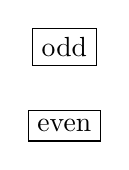
\begin{tikzpicture}[node distance = 1cm]
          \node [block]               (odd)  {\hs{odd}};
          \node [block, below of=odd] (even) {\hs{even}};
        \end{tikzpicture}
      };
      \node [block, right of=parityset] (multset) {
        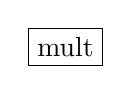
\begin{tikzpicture}[node distance = 2cm]
          \node [block] (mult) {\hs{mult}};
        \end{tikzpicture}
      };

      \path [line] (plusset)   -- (parityset);
      \path [line] (parityset) -- (multset);
    \end{tikzpicture}
    \caption{One possible topological sorting of simply connected components for
      Figure~\ref{fig:dagexample} (ignoring constructors). \hs{even} and
      \hs{odd} are mutually recursive, neither can appear before the other, so
      they are grouped into one component and handled concurrently by
      Algorithm~\ref{alg:recurrent}.}
    \label{fig:sccexample}
  \end{subfigure}
  \caption{Sorting functions from Figure~\ref{fig:coreexample} into dependency order.}
  \label{fig:dependencyexample}
\end{figure}

As an example of this recurrent process, we can consider the Peano arithmetic
functions from Figure~\ref{fig:coreexample}. A valid topological ordering is
given in Figure~\ref{fig:sccexample}, which can be our value for $d$ (eliding
Core expressions to save space):

\begin{equation}
  d = [\{(\hs{plus}, \dots)\},
       \{(\hs{odd}, \dots), (\hs{even}, \dots)\},
       \{(\hs{mult}, \dots)\}]
\end{equation}

We can then trace the execution of Algorithm~\ref{alg:recurrent} as follows:

\begin{itemize}
\item The first iteration through \textsc{RecurrentCluster}'s loop will set
  $scc \gets \{(\hs{plus}, \dots)\}$.
\item With $i = \hs{plus}$ and $e$ as its Core expression, calculating
  $featureVec(e)$ is straightforward; the recursive call $\feature{\hs{plus}}$
  will become $f_{recursion}$ (since \hs{plus} doesn't appear in $\vect{C}$).
\item The call to $kMeans$ will produce $\vect{C} \gets [\{\hs{plus}\}]$, i.e. a
  single cluster containing \hs{plus}.
\item The next iteration will set
  $scc \gets \{(\hs{odd}, \dots), (\hs{even}, \dots)\}$.
\item With $i = \hs{odd}$ and $e$ as its Core expression, the call to \hs{even}
  will result in $f_{recursion}$.
\item Likewise for the call to $\hs{even}$ when $i = \hs{odd}$.
\item Since the feature vectors for \hs{odd} and \hs{even} will be identical,
  $kMeans$ will put them in the same cluster. To avoid the degenerate case of a
  single cluster, for this example we will assume that $k = 2$; in which case
  the other cluster must contain \hs{plus}. Their order is arbitrary, so one
  possibility is $\vect{C} = [\{\hs{odd}, \hs{even}\}, \{\hs{plus}\}]$.
\item Finally \hs{mult} will be clustered. The recursive call will become
  $f_{recursion}$ whilst the call to \hs{plus} will become $2 + 3 \alpha$, since
  $\hs{plus} \in C_2$.
\item \begin{sloppypar}Again assuming that $k = 2$, the resulting clusters will
    be
    \mbox{$\vect{C} \gets [\{\hs{odd}, \hs{even}\}, \{\hs{plus},
      \hs{mult}\}]$}.\end{sloppypar}
\end{itemize}

Even in this very simple example we can see a few features of our algorithm
emerge. For example, \hs{odd} and \hs{even} will always appear in the same
cluster, since they only differ in their choice of constructor names (which are
discarded by $toTree$) and recursive calls (which are both replaced by
$f_{recursion}$).

\section{Implementation}
\label{sec:implementation}

We provide an implementation of our recurrent clustering algorithm in a tool
called \mlforhs{}~\footnote{Available at
  \url{https://github.com/warbo/ml4hsfe}}. We obtain Core ASTs from Haskell
packages using a plugin for the GHC compiler~\footnote{Available at
  \url{https://github.com/warbo/ast-plugin}}, which emits a serialised version
of each Core definition as it is being compiled. This approach is more robust
than, for example, parsing source files, since it avoids the complications of
preprocessors and language extensions altering the syntax.

A post-processing stage determines which Core definitions are suitable for
exploration, based on their visibility (whether they are encapsulated inside
their module or visible to importers), whether a data generator is available,
etc. This information, along with type signatures, arity, etc. are stored
alongside the Core definitions in JSON format.

The definitions are then sorted topologically, based on the non-local
identifiers appearing in their ASTs, and feature vectors are constructed using a
Haskell implementation of the approach described in
\S~\ref{sec:featureextraction}. Since the features associated with each
identifier may vary between iterations (as the clusters change), we leave the
raw identifiers in the vector so their features can be extracted in the correct
context.

We implement Algorithm~\ref{alg:recurrent} as a Haskell executable, which
performs the clustering and associates each Core definition with a cluster
number. These numbers are used to finish the deferred feature extraction of
identifiers, the resulting feature vectors are clustered, and the process is
repeated until all SCCs have been processed. Once the recurrent clustering is
complete, we output a JSON array of the clusters (serialised in an arbitrary
order).

\iffalse
% TODO: This seems less appropriate for this chapter, more suitable for
% Signature Selection
A separate application called \mlspec{} can read in this JSON, generate
appropriate Haskell code to invoke \quickspec{} on each cluster individually,
and evaluate that code with all appropriate dependencies installed. This
decoupling allows our feature extraction algorithm to be used for other
purposes, and allows alternative clustering involves:

\begin{itemize}
\item{Monomorphising}: If a value has polymorphic type, e.g. \hs{equal :: forall
    t. t -> t -> Bool}, we must choose a concrete representation to use (in this
  case for \hs{t}), in order to know which random generator to use. We take the
  approach used in \quickcheck{} by attempting to instantiate all type variables to
  \hs{Integer}. Any values where this is invalid, such as those with
  incompatible class constraints (e.g. \hs{forall t. IsString t => t}, where
  \hs{Integer} does not implement \hs{IsString}) will not be included in the
  signature (this is checked at the AST post-processing stage).

\item{Qualifying}: All names are \emph{qualified} (prefixed by their module's
  name), to avoid most ambiguity. There is still the possibility that multiple
  packages will declare modules of the same name, although this is rare as it
  causes problems for any Haskell programmer trying to use those modules. In
  such cases the exploration process simply aborts.

\item{Appending variables}: Once a \quickspec{} theory has been defined containing
  all of the given terms, we inspect the types it references and append three
  variables for each to the theory (enough to discover laws such as
  associativity, but not too many to overflow the limit of \quickspec{}'s exhaustive
  search).

\item{Sandboxing}: One difficulty with Haskell's packaging infrastructure is
  that all required packages and modules must be provided up-front, usually by
  specification in a Cabal file. Since \mlspec{} builds signatures
  \emph{dynamically}, depending on the cluster information it is given, we do
  not know what packages it may need. To work around this problem, we evaluate
  these strings of Haskell using a custom library called \texttt{nix-eval}. This
  uses the Nix package manager to obtain all of the required packages and make
  them available to GHC, and is described further in
  Appendix~\ref{sec:nix-eval}.

\end{itemize}

The equations resulting from evaluating these strings are collected and
outputted as JSON values, to ease further processing (e.g. displaying in some
form, sending to a theorem prover, etc.).
\fi

\section{Evaluation}
\label{sec:evaluation}

\iffalse
TODO: Alison: Next chapter? It's good to lead into the next chapter at the end
of the previous ones.
\fi

We have applied our recurrent clustering algorithm to several scenarios, with
mixed results. A major difficulty in evaluating these clusters is that we have
no ``ground truth'', i.e. there is no objectively correct way to compare
definitions. Instead, we provide a qualitative overview of the more interesting
characteristics.

As a simple example, we clustered (Haskell equivalents of) the running examples
used to present \textsc{ACL2(ml)}~\cite{heras2013proof}, shown in
Figure~\ref{fig:lisp}. These include tail-recursive and non-tail-recursive
implementations of several functions. We expect those with similar
\emph{structure} to be clustered together, rather than those which implement the
same function. The results are shown in Figure~\ref{fig:haskellcluster}, where
we can see the ``\hs{Tail}'' functions clearly distinguished, with little
distinction between the tail recursive and na\"{\i}ve implementations.

Next we tested whether these same functions would be clustered together when
mixed with seemingly-unrelated functions, in this case 207 functions from
Haskell's \hs{text} library. In fact, the \hs{helperFib} and \hs{fibTail}
functions appeared together in a separate cluster from the rest. This was
unexpected, with no obvious semantic connection between these two functions and
the others in their cluster (although most are recursive, due to the nature of
the \hs{text} library).

\begin{figure}
  \begin{common-lisp}
(defun fact (n)
  (if (zp n) 1 (* n (fact (- n 1)))))

(defun helper-fact (n a)
  (if (zp n) a (helper-fact (- n 1) (* a n))))

(defun fact-tail (n)
  (helper-fact n 1))

(defun power (n)
  (if (zp n) 1 (* 2 (power (- n 1)))))

(defun helper-power (n a)
  (if (zp n) a (helper-power (- n 1) (+ a a))))

(defun power-tail (n)
  (helper-power n 1))

(defun fib (n)
  (if (zp n)
      0
      (if (equal n 1)
          1
          (+ (fib (- n 1)) (fib (- n 2))))))

(defun helper-fib (n j k)
  (if (zp n)
      j
      (if (equal n 1)
          k
          (helper-fib (- n 1) k (+ j k)))))

(defun fib-tail (n)
  (helper-fib n 0 1))
  \end{common-lisp}
  \caption{Common Lisp functions used with \textsc{ACL2(ml)}, both
    tail-recursive and non-tail-recursive.}
  \label{fig:lisp}
\end{figure}

\begin{figure}
  \begin{haskell}
fact n = if n == 0
            then 1
            else n * fact (n - 1)

helperFact n a = if n == 0
                    then a
                    else helperFact (n - 1) (a * n)

factTail n = helperFact n 1

power n = if n == 0
             then 1
             else 2 * power (n - 1)

helperPower n a = if n == 0
                     then a
                     else helperPower (n - 1) (a + a)

powerTail n = helperPower n 1

fib n = if n == 0
           then 0
           else if n == 1
                   then 1
                   else fib (n - 1) + fib (n - 2)

helperFib n j k = if n == 0
                     then j
                     else if n == 1
                          then k
                          else helperFib (n - 1) k (j + k)

fibTail n = helperFib n 0 1
  \end{haskell}
  \caption{Haskell equivalents of the Common Lisp functions in Figure \ref{fig:lisp}.}
  \label{fig:haskelllisp}
\end{figure}

\begin{figure}
  \centering
    \tikzstyle{block} = [rectangle, draw]
    \tikzstyle{line}  = [draw, -latex']
    \begin{tikzpicture}[node distance=3cm]
      \node [block] (c1) {
        \begin{tikzpicture}[node distance = 1cm]
          \node [block]                    (factTail)  {\hs{factTail}};
          \node [block, below of=factTail] (fibTail)   {\hs{fibTail}};
          \node [block, below of=fibTail]  (powerTail) {\hs{powerTail}};
        \end{tikzpicture}
      };
      \node [block, right of=c1] (c2) {
        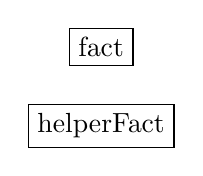
\begin{tikzpicture}[node distance = 1cm]
          \node [block]                (fact)       {\hs{fact}};
          \node [block, below of=fact] (helperFact) {\hs{helperFact}};
        \end{tikzpicture}
      };
      \node [block, right of=c2] (c3) {
        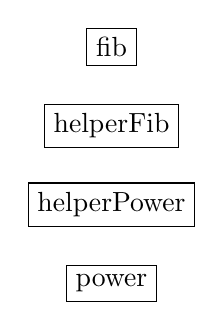
\begin{tikzpicture}[node distance = 1cm]
          \node [block]                       (fib)         {\hs{fib}};
          \node [block, below of=fib]         (helperFib)   {\hs{helperFib}};
          \node [block, below of=helperFib]   (helperPower) {\hs{helperPower}};
          \node [block, below of=helperPower] (power)       {\hs{power}};
        \end{tikzpicture}
      };
  \end{tikzpicture}
  \caption{Typical clusters for the functions in Figure \ref{fig:haskelllisp}.}
  \label{fig:haskellcluster}
\end{figure}

We have also applied our recurrent clustering algorithm to a variety of the
most-downloaded packages from \hackage{} (as of 2015-10-30), including
\texttt{text} (as above), \texttt{pandoc}, \texttt{attoparsec},
\texttt{scientific}, \texttt{yesod-core} and \texttt{blaze-html}. Whilst we
expected functions with a similar purpose to appear together, such as the
various reader and writer functions of \hs{pandoc}, there were always a few
exceptions which became separate for reasons which are still unclear.

When clustering the \hs{yesod} Web framework, the clustering did seem to match
our intuitions, in particular since all 15 of Yesod's MIME type identifiers
appeared in the same cluster.

\iffalse
Since we are working in the domain of Haskell programs, an abundant source of
statements are available in the form of \emph{tests}. For manually-written
tests, the effort required to write them implies that they must be of some
interest to their author. Many forms of test are \emph{not} suitable for our
purposes, such as \emph{unit tests} which are always trivially provable by
$\beta$-reduction; or \emph{integration tests}, which depend on the behaviour of
the external environment. One reason to study Haskell is its widespread use of
\emph{property checking}, which does give us useful data. Many Haskell property
checkers exist, based on random testing
(\quickcheck{}~\cite{claessen2011quickcheck} and
\smartcheck{}~\cite{pike2014smartcheck}), enumeration
(\smallcheck{}~\cite{runciman2008smallcheck}), observation
(\lazysmallcheck{}~\cite{reich2013advances}) and logic programming
(\sparsecheck{}~\cite{sparsecheck}).

Thankfully the major differences between these systems are in the way they
instantiate test arguments; their representations of properties are largely the
same (modulo renaming of functions and types).

Here we consider the 10 most-downloaded packages from \hackage{} (as of
2015-10-30) which have property tests; these are \texttt{warp}, \texttt{aeson},
\texttt{text}, \texttt{lens}, \texttt{conduit}, \texttt{pandoc},
\texttt{attoparsec}, \texttt{scientific}, \texttt{yesod-core} and
\texttt{blaze-html}.

% TODO: Analysis
\fi

\iffalse
Whilst recurrent clustering has produced results which merit further
investigation, the application to theory exploration has yet to be tested
empirically. This is due to \quickspec{}'s use of \quickcheck{}'s \hs{Arbitrary} type
class to generate random values for instantiating variables. Whilst we can
automatically define \quickspec{} theories and invoke them with \hs{nix-eval}, not
all types have \hs{Arbitrary} instances; those without cannot be given any
variables in our signature, which severely limits the possible combinations
which can be explored. In many cases, no variables can be included at all,
leaving just equations involving constants. This has so far prevented us from
measuring the direct impact on \quickspec{} performance, either directly by
exploring the sub-sets identified through recurrent clustering, or indirectly by
comparing the equations generated by a full brute-force search to our recurrent
clusters: those equations relating terms from different clusters would not be
discovered by our method. It is this ratio of equations found through brute
force to those found after narrowing-down by clusters which is one of our key
objectives to maximise at this stage; until we begin to pursue the
\emph{interestingness} of the properties.

The following less-serious problems were also encountered while applying
\mlforhs{} to \hackage{} packages:

\begin{itemize}
\item Some packages, such as \texttt{warp} and \texttt{conduits}, get no
  declarations to cluster. This is because they make all of their declarations
  privately, e.g. in ``internal'' modules, then use separate modules to export
  the public declarations. GHC's renaming phase makes all references to such
  exports canonical, by pointing them to the private declarations. This forces
  us to ignore such declarations, as \quickspec{} will not be able to access them.

\item Since we do not support type-level entities, we ignore type
  classes. Unfortunately, this also means ignoring any value-level bindings (AKA
  ``methods'') which occur in a type class instance. Instead of being clustered,
  these result in references getting $f_{recursion}$ features. This is
  especially noticable in libraries like \hs{scientific}, where only the
  functions for constructing and destructing numbers in scientific notation are
  clustered; all of the arithmetic is defined in type classes. One difficulty
  with supporting methods is that their namespace in Core is disjoint from that
  of regular Haskell identifiers: a transformation layer would be required,
  along with explicit type annotations to avoid ambiguity.
\end{itemize}
\fi

It seems like this recurrent clustering method has promise\iffalse TODO: Alison: Informal, vague \fi, although it will
require a more thorough exploration of the parameters to obtain more intuitively
reliable results. These clusters can then be used in several ways to perform
theory exploration; the most na\"{\i}ve way being to explore each cluster as
\quickspec{} signature in its own right, which we investigate as a potential
solution to the Signature Selection problem.

\iffalse
TODO: Alison: Next chapter? It's good to lead into the next chapter at the end of the previous ones.
\fi

\iffalse
As alluded to previously, we also have the opportunity to reason by
\emph{analogy}. Similar to the work on ACL2(ml) \cite{heras2013proof}, we could
produce a general ``scheme'' from each equation we find (either through \quickspec{}
or by data mining test suites); like Isabelle approaches have shown
\cite{Montano-Rivas.McCasland.Dixon.ea:2012}, these schemes could then be
instantiated to a variety of similar values, in an attempt to find new theorems
which are analogues of existing results from a different context. ``Mutating''
existing theorem statements in such a way would also increase the chance of any
result being considered interesting; since it's likely that the unmodified
statement was deemed interesting, and the new result would not in general follow
as a simple logical consequence.
\fi

\iffalse
\subsection{Recurrent Clustering}
\label{sec:clusteringexpressions}

Our recurrent clustering algorithm is similar to that of ML4PG, as our
transformation maps the elements of a syntax tree to distinct cells in a
matrix. In contrast, the matrices produced by ACL2(ml) \emph{summarise} the tree
elements: providing, for each level of the tree, the number of variables,
nullary symbols, unary symbols, etc.

Unlike ML4PG, our algorithm can handle mutually-recursive definitions, but it
also ignores types. This is because obtaining the type of each component of a
Core definition is more difficult than in ML4PG (which queries the current
\textsc{Proof General} state), and is left for future work.

The way we \emph{use} our clusters to inform theory exploration is actually more
similar to that of ACL2(ml) than ML4PG. ML4PG can either present clusters to the
user for inspection, or produce automata for recreating proofs. In ACL2(ml), the
clusters are used to restrict the search space of a proof search, much like we
restrict the scope of theory exploration.

\section{Conclusion and Future Work}
\label{sec:conclusion}

Our use of clustering to pre-process \quickspec{} signatures has required many
decisions and tradeoffs to be made. Hence our approach is just one possibility
out of many alternatives which could be investigated to push this work further.

The most obvious next step is to incorporate types. Types contain valuable
information about an expression, and would allow us to distinguish between
constructors. Since our algorithm closely follows that of ML4PG, which
\emph{does} support types, the only barrier is the practical issue of
propagating annotations through all of the Core definitions.

More speculative directions include the use of \emph{learned} representations,
rather than our hand-crafted features \cite{bengio2013representation}. This
would provide an interesting comparison, as well as being more robust in the
face of language evolution. Another intriguing possibility is to extend the
recurrent nature of our algorithm to make use of the discovered properties
during clustering; for example, by treating the discovered equations as rewrite
rules to reduce the ASTs prior to feature extraction.
\fi
W
